\documentclass[projektplan/plan.tex]{subfiles}
\begin{document}
\section{Organisationsplan för hela projektet}

\begin{figure}[h]
    \centering
    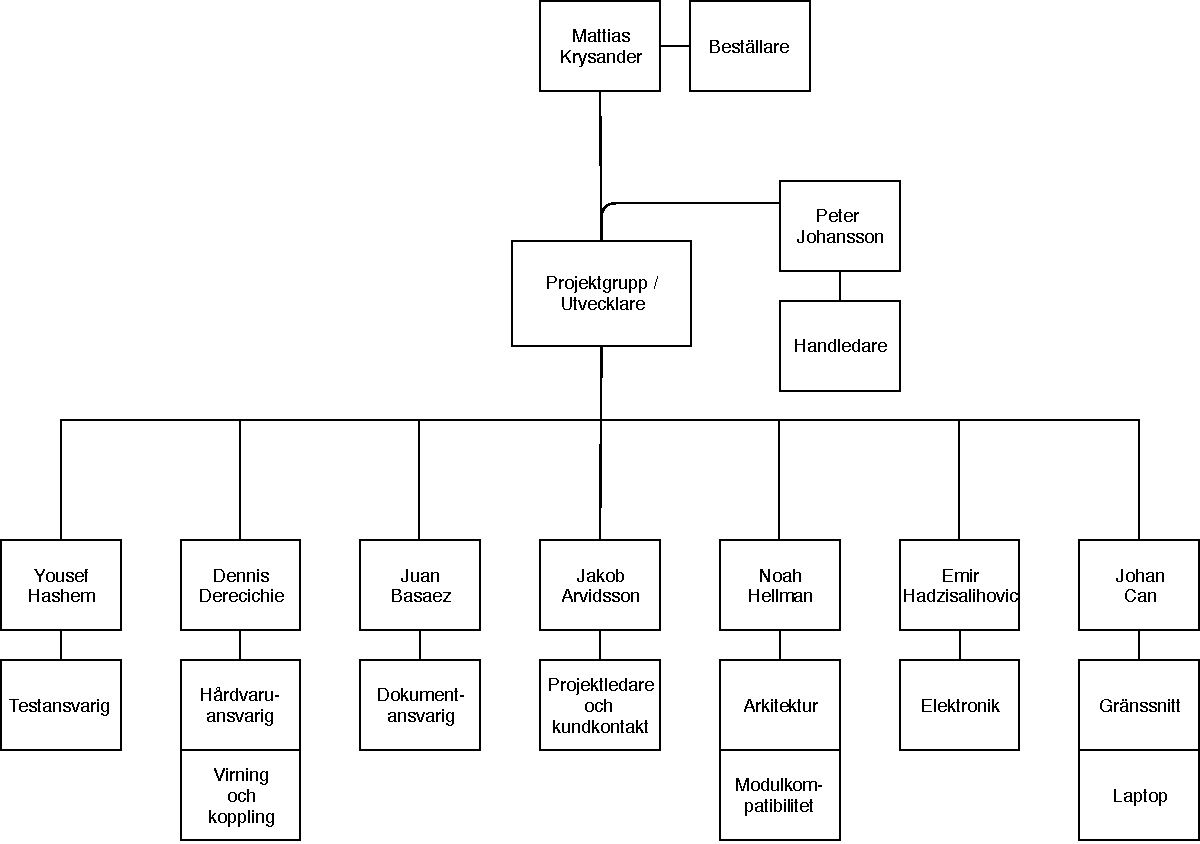
\includegraphics[width=0.6\linewidth]{projektplan/figures/orgplan.pdf}
    \caption{Övergripande bild över organisationsstrukturen}
    \label{fig:orgplan}
\end{figure}
\noindent
Här beskrivs hur gruppen kommer att organisera arbetet under projektets gång.
Bland annat är planen att gruppen ska sträva efter att dela upp arbetet till
små grupper. Eftersom det finns tre moduler så är själva planen att gruppen
delas upp i tre grupper där vardera grupp arbetar med sin egen modul. Vid
kritiska delar, t.ex där alla moduler är beroende till att något ska vara
färdigt så ska gruppen tillsammans lösa detta. Om en grupp stöter på hinder så
ska gruppen hjälpas åt att tillsammas lösa problemet. Figur \ref{fig:orgplan}
visar strukturen på organisationen. Under projektgruppen är alla utvecklare
listade med respektive ansvarsområden.  

\noindent
\begin{minipage}{\textwidth}
\subsection{Villkor för samarbetet inom projektgruppen}
\label{sec:doc}
Nedan följer en lista av de punkter gruppen har enats om att följa vid samarbete.
{\renewcommand{\arraystretch}{1.6}
\begin{longtable}{p{0.75\textwidth}p{0.20\textwidth}}
    \bfseries Fråga &
    \bfseries Inställning \\\hline
    Alla deltagare i gruppen ska delta vid de tillfällen som gruppen kommit
    överens om. &
    Instämmer helt
    \\
    Alla deltagare i gruppen ska komma väl förberedda till sammankomsten. &
    Instämmer delvis
    \\
    Det är viktigt med en ”samordnare” i gruppen. &
    Instämmer helt
    \\
    Arbetsuppgifterna ska fördelas likvärdigt mellan gruppmedlemmarna, så att
    tid- och arbetsinsatsen blir ungefär lika stor. &
    Instämmer helt
    \\
    När vi arbetar i gruppen ska vi hålla oss till fakta och undvika prat om
    känslor och personliga erfarenheter. &
    Instämmer delvis
    \\
    Samarbetet i gruppen måste när som helst kunna diskuteras öppet, även om
    det innebär obehag för någon. &
    Instämmer helt
    \\
    Den som inte bidrar aktivt ska inte heller dra nytta av gruppens gemensamma
    arbete. &
    Instämmer delvis
    \\
    Det är viktigt att ge varandra återkoppling, såväl positiv som negativ. &
    Instämmer helt
    \\
    Varje träff avslutas med en utvärdering, där var och en belyser hur arbetet
    i gruppen fungerat. &
    Tar helt avstånd
    \\
    Vår grupps ambitionsnivå är att arbetet ska leda till att det framtagna
    resultatet i projektet blir det bästa tänkbara. &
    Instämmer delvis
    \\
\end{longtable}}
\end{minipage}

\newpage
\subsection{Definition av arbetsinnehåll och ansvar}
Vad som anses vara en bra arbetsinsats definieras av majoriteten i gruppen.
Ansvar i gruppen är att man ska vara ärlig mot varandra och vid begäran ge en
ärlig återkoppling om hur arbetet har gått. Om man står för en viss
konstruktion som inte fungerar så bär man ansvaret att se till att informera
gruppen. Därefter har man ansvar att rätta felet eller att be om hjälp där man
ska förklara hur konstruktionen är tänkt att fungera.

Varje medlem skall speciellt se till att de aktiviteter inom deras
anvsarsområde blir utförda. Om en medlem är frånvarande skall närvarande
medlemmar se till att medlemmens anvsarsområde blir genomfört. Ansvarsområdena
definieras nedan.

\begin{labeling}{lååååååång titeeeeel}
    \item[Arkitekt] Ska se till att kraven blir uppfyllda genom utvärdering.
        Arkitekten bestämmer arkitekturen på en hög nivå och vilka komponenter
        som ska användas. Arkitekten har sista ordet i tekniska frågor.

    \item[Projektledare] Ska se till projektets mål möts genom att planera och
        leda projektets arbete. Projektledaren skriver tids- och
        statusrapporter. Ledaren är kundansvarig och sköter all kommunikation
        med beställaren. Har sista ordet i alla frågor, utöver tekniska frågor.

    \item[Testansvarig] Utvärderar kraven med hjälp av tester och bestämmer när
        testningen är tillräcklig. Den testansvarige ska planlägga tester och
        se till att de blir utvecklade. Den testansvarige skall ge återkoppling
        till projektgruppen utifrån testerna.

    \item[Dokumentansvarig] Ansvarar för att alla dokument enligt
        dokumentplanen utförs och blir levererade.

    \item[Gränssnittanvsarig] Designar användargränssnittet på fjärrklienten
        och ser till att det blir utvecklat.

    \item[Hårdvaruansvarig] Ser till att implementationen och virningen av
        hårdvara är korrekt.

    \item[Elektronikansvarig] Anvsarar för designen av kretscheman, och den
        elektroniska delen av implementationen.
\end{labeling}

\end{document}
